\section{\scshape Proposal}\label{sec:proposal}

\subsection{Research questions}
\begin{frame}{Research questions}
	\begin{itemize}
		\item How to reliably learn new assembly skills given that the tracking of the assembly objects will always have pose estimation errors and temporary occlusions by the operator?
			\item How to automatically extract assembly information from CAD / SOP data?
		\item How to generalize a specific assembly skill and reuse it to perform similar tasks?
		\item How to efficiently coordinate complex assembly procedures between humans and robots in a shared work space?
	\end{itemize}
\end{frame}

\subsection{Objectives}
\begin{frame}{Objectives}
	\begin{itemize}
		\item Development of a cooperative assembly system capable of:
		\begin{itemize}
			\item Reliably learning by human demonstration
			\item Perform cooperative assembly tasks with human operators
			\item Help human operators perform their tasks faster by projecting assembly information into the workspace
			\begin{itemize}
				\item Showing which objects the human should pick up
				\item Where to place the objects with precision (no need for manual measurements)
				\item The order of assembly
			\end{itemize}
		\end{itemize}

	\end{itemize}
\end{frame}

\subsection{Applications}
\begin{frame}{Applications}
	\begin{itemize}
		\item Assembly of objects with increasing complexity, such as:
		\begin{itemize}
			\item Alternators
			\item Engines
			\item Gearboxes
		\end{itemize}
	\end{itemize}
	\begin{figure}[!ht]
		\centering
		\begin{minipage}{0.32\textwidth}
			\centering
			\includegraphics[height=.28\textheight]{gearbox}
			\caption{Gearbox parts}
		\end{minipage}%
		\begin{minipage}{.32\textwidth}
			\centering
			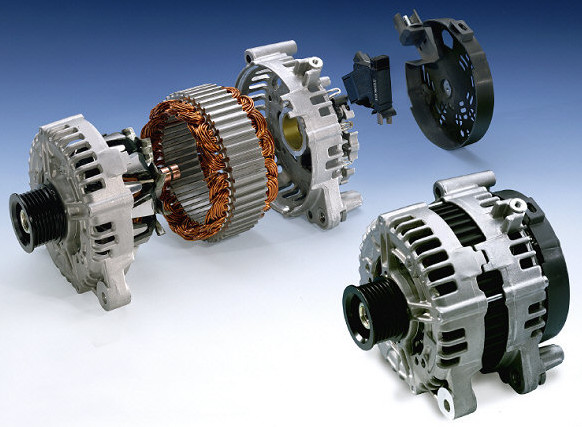
\includegraphics[height=.28\textheight]{alternator}
			\caption{Alternator parts}
		\end{minipage}%
		\begin{minipage}{0.32\textwidth}
			\centering
			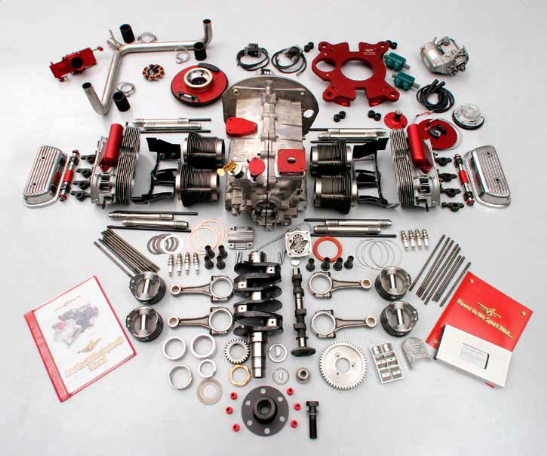
\includegraphics[height=.28\textheight]{engines}
			\caption{Engines parts}
		\end{minipage}
	\end{figure}
\end{frame}

\subsection{Methodology}
\begin{frame}{Methodology}
	\begin{itemize}
		\item Detailed description of the intended functionality and final users of each software module
		\item Selection of the hardware and software platform in which the research will be performed
		\item Selection / creation of representative testing datasets for each of the main software modules
		\begin{itemize}
			\item 2d / 3D perception of geometry / objects and operator movements
			\item Learning new skills
			\item Human Machine Interface
		\end{itemize}
		\item Test and comparison of current state of the art methods for each software module
		\item Development of new / improved methods / algorithms when required
		\item Focus research on reliably learning new assembly skills
		\item Industrial testing of each software module with the final users
	\end{itemize}
\end{frame}
